% Chapter Template

\chapter{Empirical Study} % Main chapter title

\label{Chapter4} % Change X to a consecutive number; for referencing this chapter elsewhere, use \ref{ChapterX}

%----------------------------------------------------------------------------------------
%	SECTION 1
%----------------------------------------------------------------------------------------
\section{Study Design}\label{sec:studydesign}

The aim of this paper is to provide information about some of the most used automatic exploration tools for android applications inside the industry and the academy. This information is going to be useful for developers and researchers when they face a decision-making situation related to the selection of the right exploration tool that fits their needs. In consequence, an empirical study was designed and will provide answers for the following research questions: 

\begin{itemize}

\item RQ-1 What tool reaches the highest accumulated method coverage?
\item RQ-2 What tool finds the largest number of failures during the explorations?
\item RQ-3 what tool has the top average value of errors found across different apps?
\end{itemize}

\section{Context of the Study}

With the purpose of answering the research questions, 11 applications where selected to be executed. The list of selected apps can be seen in Figure.\ref{tab:apps}. This set is a subset of a set of open source applications widely used by  The Software Design Lab for other studies and tests. Every APK in the subset should be successfully instrumented by InstruAPK, it should compile without any problem after instrumentation and it should be launched in an emulator without any issue after the instrumentation process.

Equally important, four exploration tools were selected, two from the industry and two from the academic side. The first tool is Firebase Test Lab (Section \ref{sec:testlab}). It was selected for being widely used in industry and for also being a Google product. The second one, Monkey \footnote{https://developer.android.com/studio/test/monkey}, was selected as a baseline because it is the state-of-the-art and practice tool for inputs generation; it is by default included in the Android SDK Tools. The third one, Droidbot (Section \ref{sec:droidbot}), was selected from the academic side. Droidbot has been a point of study for many researches. Many others tools have based their functionality on this tool. The last one is RIP (Section \ref{sec:rip}), this tool was selected for being of special interest for us. It is our own exploration tool and it is currently an active project inside the Software Design Lab at University of Los Andes. 

Each tool was executed ten times per application and with a maximum time of 30 minutes. The number of executions and the maximum time were arbitrary decisions that were made because of time limitations for the study. During the study we noticed that most of the tools ended the exploration or reached their maximum coverage within the first 15 minutes. Which means that the maximum time for exploration was more than enough in almost all cases. 

The same emulator was used for all the exploration tools, except for Firebase Test Lab because this tool offers its own set of emulators. In all the cases a Pixel 2 XL was used, but in the cases of Monkey, Droidbot and RIP there was more control over the device specifications. For the case of the last mentioned tools the specifications of the emulator used within the experiment are:  Google APIs Intel Atom (x86), API level 27, SD card size of 512MB, and RAM size of 4096MB. The specifications are unknown for the case of Test Lab.

\begin{table}[t]
	\centering
	\caption{Applications used for the study}
	\label{tab:apps}
	\resizebox{\textwidth}{!}{
		\begin{tabular}{c c c c}
			App ID & Package Name & \# Methods Reported by APKAnalyzer & \# Methods Instrumented by InstruAPK\\
			\hline
			1 & appinventor.ai\_nels0n0s0ri0.MiRutina & 61993 & 9351\\
			2 & com.evancharlton.mileage & 4000 & 1162\\
			3 & com.fsck.k9 & 18799 & 7003\\
			4 & com.ichi2.anki & 32370 & 2209\\
			5 & com.workingagenda.devinettes & 19274 & 66 \\
			6 & de.vanitasvitae.enigmandroid & 13083 & 574 \\
			7 & info.guardianproject.ripple & 19429 & 100 \\
			8 & org.connectbot & 20606 & 1145\\
			9 & org.gnucash.android & 75473 & 504\\
			10 & org.libreoffice.impressremote & 14691 & 649\\
			11 & org.lumicall.android & 45784 & 540\\
			\hline
		\end{tabular}
	}
\end{table}

Finally, the work flow specified in Section \ref{sec:generalApproach} was followed for each application by using the aforementioned exploration tools. 

\section{Results}\label{sec:results}

\subsection{Method Coverage Results}\label{sec:coverageResults}

As mentioned before, some explorations ended before the max execution time allowed (30 minutes) giving no data for the upcoming seconds. To solve this scenarios, the coverage reached by the tool at the moment when the exploration ends, was kept the same until completing the total time. Once this have been done, the results are comparable second by second.


As a result of the instrumentation made by InstruAPK, the timestamp of every called method is known, thus, the coverage reached by a tool in a specific second can be calculated. The aforementioned information was used to calculate the average accumulated method coverage reached for every tool across the 11 analysed apps. Such results are presented in figure \ref{fig:averageCoverageInstruAPK} and figure \ref{fig:averageCoverageAPKAnalyzer}. The data were calculated as follow:

\begin{enumerate}
\item For every exploration of an application add the coverage reached for tool second by second without adding the results of the previous seconds.
\item Divide by the number of explorations by tool. (This results in the average method coverage reached by a tool in one application)
\item Add the results of the previous step. (By tool)
\item Divide by the number of applications (This will end in the average method coverage of a tool for all the applications)
\end{enumerate} 

For calculating this, both data were used, the method coverage calculated by using the number of instrumented methods reported by InstruAPK and the number of methods reported by APKAnalyzer. The curves have the same behaviour, as expected, but in Figure \ref{fig:averageCoverageAPKAnalyzer} gap between tools is more visible.

\begin{figure}[h]
\centering
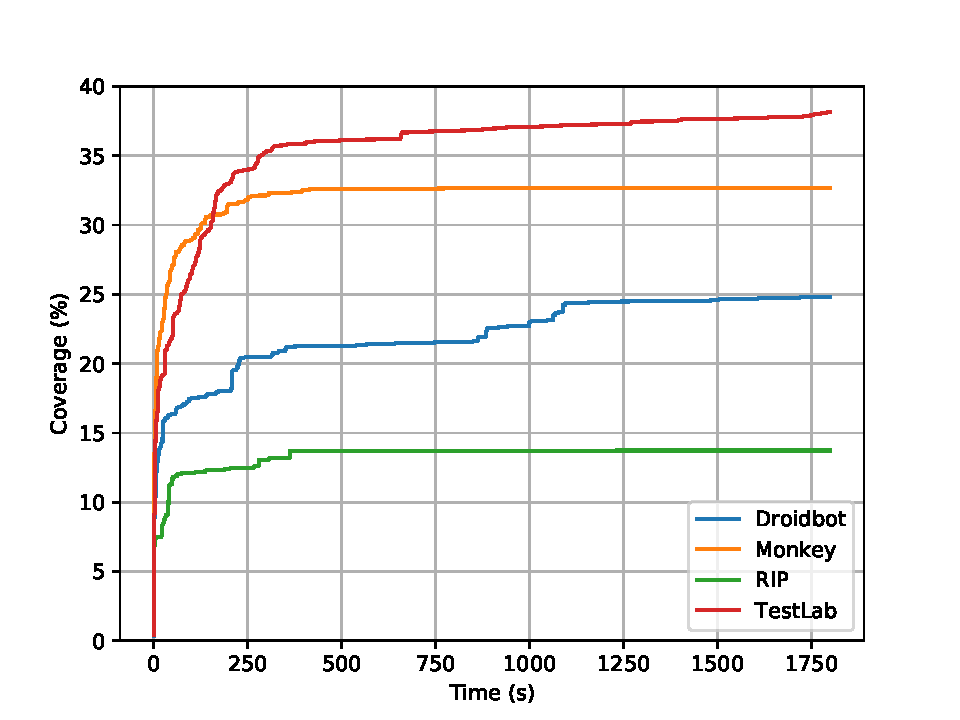
\includegraphics[width=0.8\textwidth]{../Figures/averageCoverageInstruAPK.pdf}
\caption{Average Accumulated Method Coverage by Tool According to the Number of Instrumented Methods Reported by InstruAPK}\label{fig:averageCoverageInstruAPK}
\end{figure}

\begin{figure}[h]
\centering
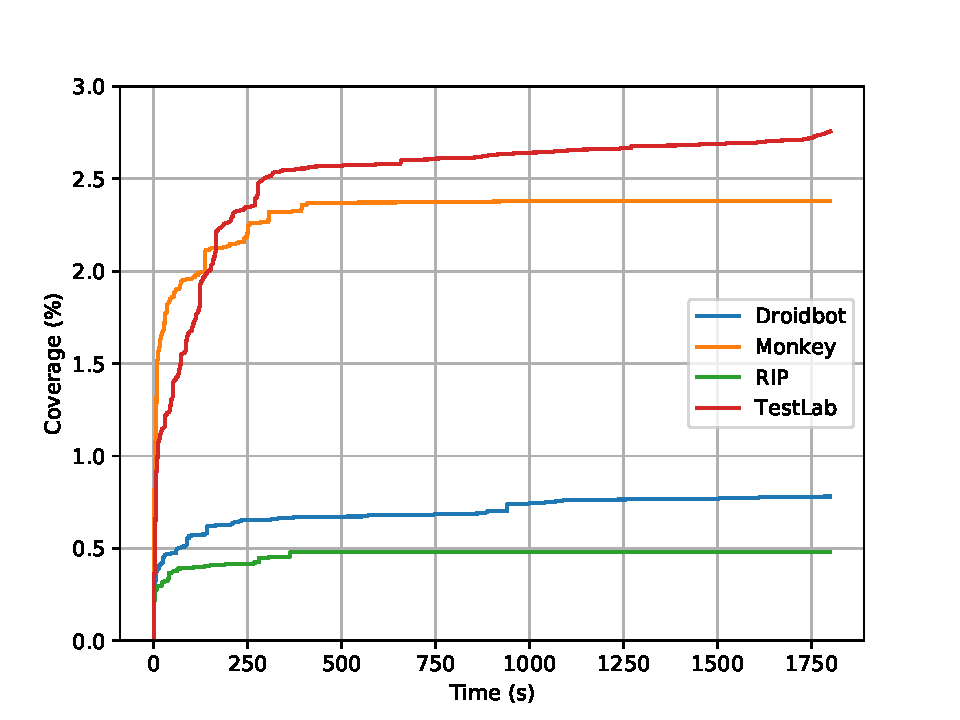
\includegraphics[width=0.8\textwidth]{../Figures/averageCoverageAPKAnalyzer.pdf}
\caption{Average Accumulated Method Coverage by Tool According to the Number of Methods Reported by APKAnalyzer}\label{fig:averageCoverageAPKAnalyzer}
\end{figure}

\MARIO{Terminar de escribir aquí ahora que no hay RQ-1}

The answer for RQ-1 can be seen easily in figure \ref{fig:averageCoverageInstruAPK} or figure \ref{fig:averageCoverageAPKAnalyzer}. Firebase Test Lab is the tool with the highest average method coverage reached. Surprisingly, followed by Monkey, even when monkey has no complex architecture nor exploration strategy, it has the second highest average method coverage within this study.

For answering RQ-2 is know that, for every execution the called methods are stored, every method has an unique id that was given during the instrumentation. Thus, after the 10 executions of an application, the result of every execution is analysed searching for the methods that have not been called neither during previous explorations nor during the current one. Therefore, the number of unique methods called in that application is obtained. That is what is named as accumulated coverage. This results can be seen in figure \ref{fig:boxplotAccumulated}. The coverage presented in figure \ref{fig:boxplotAccumulated} was calculated using the number of instrumented methods reported by InstruAPK. 

\begin{figure}[h]
\centering
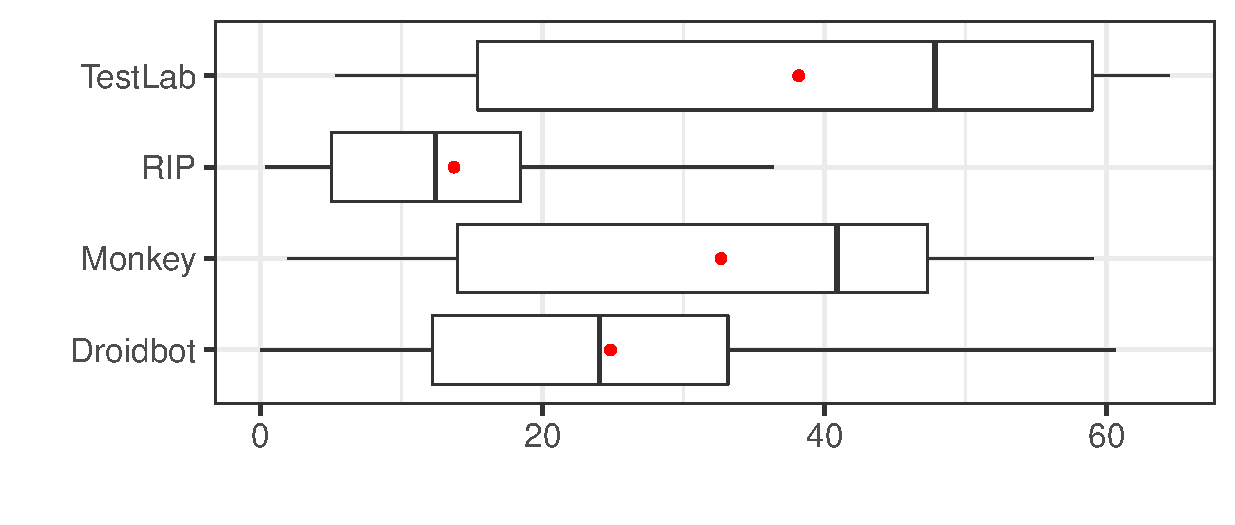
\includegraphics[width=0.8\textwidth]{../Figures/boxplotAccumulated.pdf}
\caption{Boxplot of Accumulated Coverage by Tool}\label{fig:boxplotAccumulated}
\end{figure}

So, again, the tool at first place is Firebase Test Lab, but this time, the second tool with the highest value is Droidbot.

\subsection{Error Results}\label{sec:errorResults}

Two different values for the errors were calculated. first, the total number of different error traces found by a tool throughout all the explorations (see Figure \ref{fig:maxerrors}). The second one, shown in Figure \ref{fig:averagaerrors}, is the average number of errors found by tool throughout all the explorations. 

\begin{figure}[h]
\centering
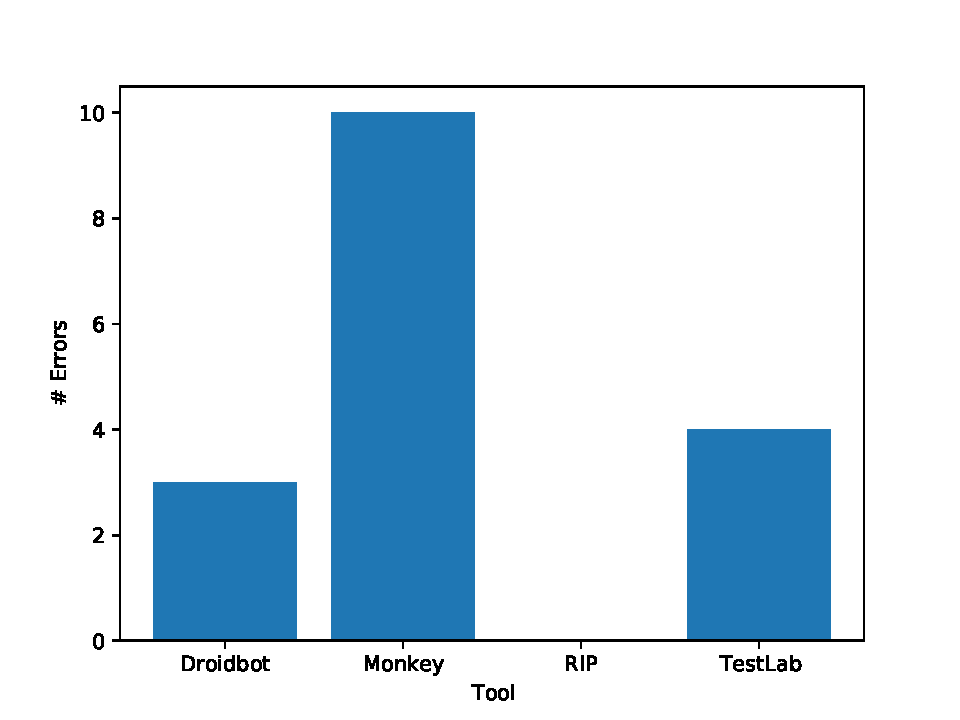
\includegraphics[width=0.8\textwidth]{../Figures/maxErrors.pdf}
\caption{Maximum Number of Errors Found by Tool}\label{fig:maxerrors}
\end{figure}

\begin{figure}[h]
\centering
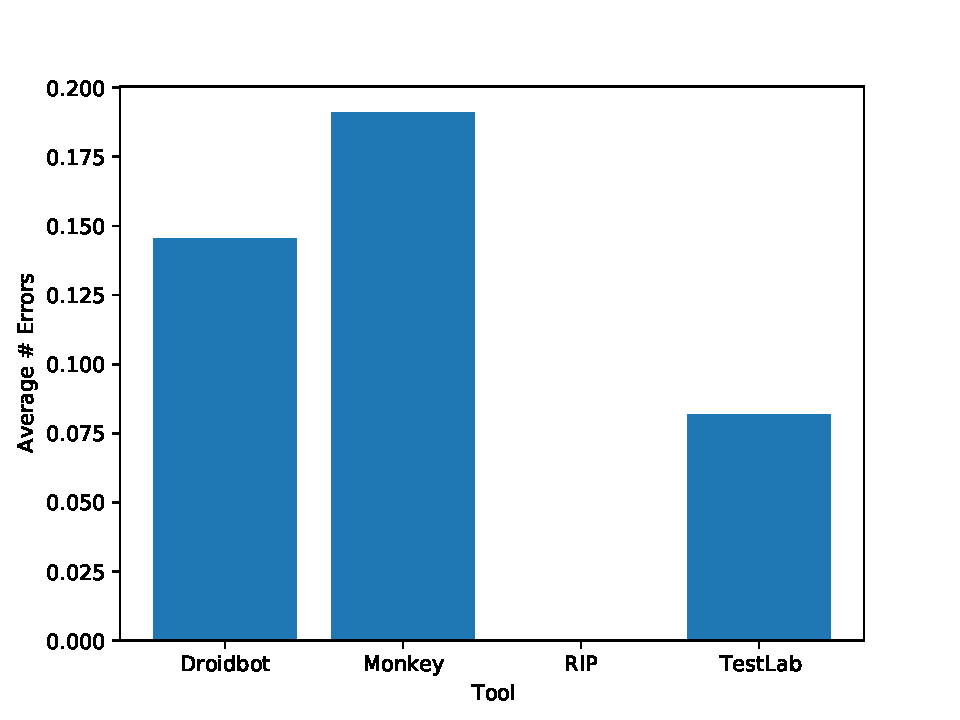
\includegraphics[width=0.8\textwidth]{../Figures/averageErrors.pdf}
\caption{Average Number of Errors Found by Tool}\label{fig:averagaerrors}
\end{figure}

These numbers were extracted by CoverageAnalyzer (Section \ref{sec:ca}). The numbers includes android runtime exceptions as well as exceptions. The tool searches for stack traces in the logcat file and filters the results using the package name of the tool under analysis. 

This data give the responses for RQ-3 and RQ-4. Which in both cases is Monkey.\MARIO{Say explicitly the answer to the questions}

